%
%===============>>  ГРУППА 8-1 МОДУЛЬ 8  <<=============
%
\setmodule{9}

%BEGIN_FOLD % ====>>_____ Занятие 1 _____<<====
\begin{class}[number=1]
	\begin{listofex}
		\item 
		\begin{minipage}[t]{\bodywidth}
			На рисунке \( AB = 4 \), \( BE = 8 \), \( DE = 5 \), прямая \( AB \) перпендикулярна прямой \( BD \), \( CD \) перпендикулярна \( BD \) и \( EA \) перпендикулярна \( EC \).	Найдите \( CD \). 
		\end{minipage}
		\hspace{0.02\linewidth}
		\begin{minipage}[t]{\picwidth}
			% TODO: \usepackage{graphicx} required
			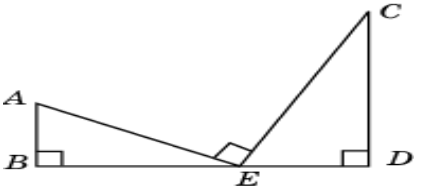
\includegraphics[align=t, width=\linewidth]{../../../../exercises/lists/pics/G81M9L1-1}
		\end{minipage}
		\item 
		\begin{minipage}[t]{\bodywidth}
			На рисунке \( DE = 10 \), \( CE = 8 \), \( BC = 12 \), угол \( BAC \) равен углу \(  EDC \). Найдите \( AB \).
		\end{minipage}
		\hspace{0.02\linewidth}
		\begin{minipage}[t]{\picwidth}
			% TODO: \usepackage{graphicx} required
			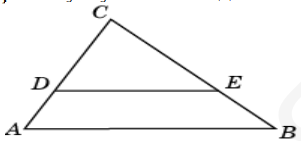
\includegraphics[align=t, width=\linewidth]{../../../../exercises/lists/pics/G81M9L1-2}
		\end{minipage}
		\item Через точки \( M \) и \( N \), принадлежащие сторонам \( AB \) и \( BC  \) треугольника \(  ABC \) соответственно, проведена прямая \( MN \), параллельная стороне \( AC \). Найдите длину \( CN \), если \( BC = 6 \), \( MN = 4 \) и \( AC = 9 \).
		\item  Прямая, параллельная основанию треугольника, делит его на треугольник и трапецию, площади которых относятся как 4:5. Периметр образовавшегося треугольника равен 20 см. Найдите периметр данного треугольника.
		\item Через вершину прямого угла прямоугольного треугольника с катетами 6 и 8 см проведен перпендикуляр к гипотенузе. Вычислите площади образовавшихся треугольников.		
		\item  В прямоугольном треугольнике \( ABC \) проведена высота \( CH \) к гипотенузе. \( CH=4 \), \( BH=3 \). Найдите катет \( AC \).		
		\item  Основание треугольника 15 см, а боковые стороны 13 и 14 см. Высота разделена в отношении 2:3 (считая от вершины) и через точку деления проведена прямая, параллельная основанию. Найдите площадь образовавшейся при этом трапеции. 
		\item Подобны ли треугольники \( ABC \) и \( A_1B_1C_1 \), если известно, что:
		
		\begin{tasks}(1)
			\task \( AB = 10 \) см; \( BC = 5 \) см; \( AC = 7 \) см; \( A_1B_1 = 15 \) см; \( B_1C_1 = 7,5 \) см; \( A_1C_1 = 9,5 \) см?
			\task \( \angle A = 37\degree \), \( \angle B = 48\degree \), \( \angle C_1 = 95\degree \), \( \angle B_1 = 48\degree \)?
			\task 	\( AB = 10  \) см, \( BC = 8 \) см, \( A_1B_1 = 5 \) см, \( A_1C_1 = 3 \) см, \( \angle C = \angle C_1 = 90\degree \)?
		\end{tasks}
		\item В прямоугольном треугольнике проведена высота к гипотенузе. Гипотенуза треугольника делится этой высотой на отрезки длиной 9 и 289. Найдите эту высоту и катеты треугольника.
		\item В прямоугольном треугольнике катет равен 4, а проекция этого катета на гипотенузу равна 2. Найдите гипотенузу, второй катет и его проекцию на гипотенузу.
		\item \( M \) и \( K \) соответственно середины сторон \( AB \) и \( BC \) треугольника \( ABC \). Найдите \( MK \), если \( AC = 7 \) см.
		\item В треугольнике \( ABC \) \( О \) и \( P \) --- середины сторон \( BC \) и \( AC \) соответственно. Длина отрезка \( OP \) равна 2,7 см. Найдите \( AB \).
		
	
	\end{listofex}
\end{class}
%END_FOLD

%BEGIN_FOLD % ====>>_____ Занятие 2 _____<<====
\begin{class}[number=2]
	\begin{listofex}
		\item 
		\begin{minipage}[t]{\bodywidth}
			В прямоугольном треугольнике биссектриса острого угла делит катет на отрезки \( 10 \) см и \( 6 \) см. Найдите периметр треугольника.
		\end{minipage}
		\hspace{0.02\linewidth}
		\begin{minipage}[t]{\picwidth}
			% TODO: \usepackage{graphicx} required
			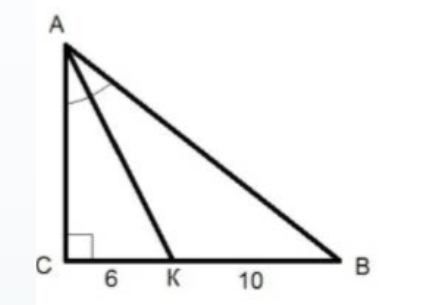
\includegraphics[align=t, width=\linewidth]{../../../../exercises/lists/pics/G81M9L2-1}
		\end{minipage}
	\item 
	\begin{minipage}[t]{\bodywidth}
		Определить длину \( AD\) геометрической фигуры на рисунке.
	\end{minipage}
	\hspace{0.02\linewidth}
	\begin{minipage}[t]{\picwidth}
		% TODO: \usepackage{graphicx} required
		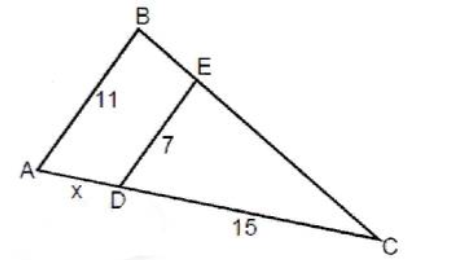
\includegraphics[align=t, width=\linewidth]{../../../../exercises/lists/pics/G81M9L2-2}
	\end{minipage}
	\item В прямоугольном треугольнике \( ABC \) высота, проведенная к гипотенузе \( AB \), делит ее на части, разность длин которых равна \( 6 \) см, а высота \( CH \) равна \( 4 \). Вычислите длину гипотенузы.
	\item В равнобедренном треугольнике \( ABC \) высота \( AE \), опущенная на боковую сторону, делит ее на отрезки \( 7 \) см и \( 2 \) см, считая от вершины. Вычислите основания треугольника.
	\item Биссектриса \( AD \) угла треугольника \( ABC \) делит противоположную сторону на отрезки \( 7 \) см и \( 5 \) см. Периметр треугольника равен \( 36 \) см. Вычислите стороны треугольника.
	\item В треугольнике АВС высота \( СН \) и медиана \( СМ \) делят угол \( С \) на три равные части. Докажите, что угол \( С \) – прямой.
	\item Точка \( E \) лежит на стороне \( AC \) треугольника \( ABC \), причём \( \dfrac{EC}{AE} = 2 \). Точка \( D \) лежит на \( BC \), причём \( ED\parallel AB \). Найдите \( AB \), если \( ED = \dfrac{4}{3} \).
	\item 
	\begin{minipage}[t]{\bodywidth}
		 Дан прямоугольный треугольник  \( \Delta ABC\)  \( \angle C = 90\degree  \), \( CH \) – высота. \( AH=9 \), \( BH = 16 \). Найти \( BC \), \( AC \), \( CH \).
	\end{minipage}
	\hspace{0.02\linewidth}
	\begin{minipage}[t]{\picwidth}
		% TODO: \usepackage{graphicx} required
		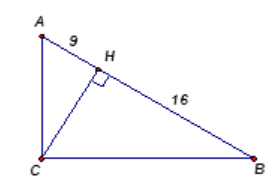
\includegraphics[align=t, width=\linewidth]{../../../../exercises/lists/pics/G81M9L2-3}
	\end{minipage}
	\item Найдите периметр прямоугольного треугольника, высота которого делит гипотенузу на отрезки длиной \( 4,5 \) см и \( 8 \) см.
	\item В треугольнике, стороны которого равны \( 15 \), \( 20 \), \( 25 \), проведена высота к его большей стороне. Найдите отрезки, на которые высота делит эту сторону.
	\end{listofex}
\end{class}
%END_FOLD

%BEGIN_FOLD % ====>>_ Домашняя работа 1 _<<====
\begin{homework}[number=1]
	\begin{listofex}
		\item Решите уравнения: 
		\begin{tasks}(2)
			\task \( 12 - x^{2} =11 \)
			\task \( x^{2} - 10x =0 \)
		\end{tasks}
		\item Решите уравнения: 
		\begin{tasks}(2)
			\task \(  x^{2} - 5x+4=0 \)
			\task \(  x^{2} - 5 =(x+5)(2x – 1)\)
		\end{tasks}
		\item Решите уравнения: 
		\begin{tasks}(2)
			\task \(  3x^{4}-18x^{2}+27=0 \)
			\task \(  -5y^{4}+30y^{2}-40=0\)
		\end{tasks}
		\item Прямоугольный газон обнесен изгородью длиной 30 м. Площадь газона 56 м\( ^{2} \). Найдите длины сторон. 
		\item При каких значениях \( k \) уравнение \( x^{2} + 2x + k = 0 \)  имеет один  корень?
		\item Число \( -6 \) является корнем уравнения \( 2x^{2} + bx - 6 = 0 \). Найдите второй корень уравнения и значение \( b \).
	\end{listofex}
\end{homework}
%END_FOLD

%BEGIN_FOLD % ====>>_____ Занятие 3 _____<<====
\begin{class}[number=3]
	\begin{listofex}
		\item Решите уравнения:
		\begin{tasks}(2)
			\task \( x^{4}-24x^{2}-25=0 \)
			\task \( x^{4}-12x^{2}-64=0 \)
			\task \( x^{4}-8x^{2}-9=0 \)
			\task \( x^{4}-2x^{2}-8=0 \)
		\end{tasks}
		\item Решите уравнения:
		\begin{tasks}(1)
			\task \( (x^{2}-2)^{2}+16(x^{2}-2)-161=0 \)
			\task \( (x^{2}-9)^{2}+8(x^{2}-9)-105=0 \)
			\task \( (x^{2}+3)^{2}-32(x^{2}+3)-273=0 \)
		\end{tasks}
		\item Решите уравнения: \begin{tasks}(2)
			\task \( (x^{2}-9)^{2}-4(x^{2}-9)+3=0 \)
			\task \( (x^{2}+x+1)(x^{2}+x+2)=12 \)
			\task \( (x^{4}-5x^{2})^{2}-2(x^{4}-5x^{2})=24 \)
			\task \( (x^{2}-6x)^{2}-2(x-3)^{2}=81 \)
			\task \( (x^{2}+3x)^{2}-4(x^{2}+3x+8)=0 \)
			\task \( (x^{2}+8x)(x^{2}+8x-6)=280 \)
		\end{tasks}
		
	\end{listofex}
\end{class}
%END_FOLD

%BEGIN_FOLD % ====>>_____ Занятие 4 _____<<====
\begin{class}[number=4]
	\begin{listofex}
		\item Найдите корень уравнения \begin{tasks}(2)
			\task \( 1-7(4+2x)= -9-4x \)
			\task \( 8-5(2x-3)=13-6x \)
		\end{tasks}
		\item Решите системы уравнений:
		\begin{tasks}(2)
			\task \( \begin{cases}
				x-2y=-9\\\ y=3x+2
			\end{cases} \)
			\task \( \begin{cases}
				2y+x=-9\\\ 5x-4y=16
			\end{cases} \)
			\task \( \begin{cases}
				4-x=y+5\\\ y-4x=14
			\end{cases} \)
			\task \( \begin{cases}
				3x+y=14\\\ 5x=3y
			\end{cases} \)
			\task \( \begin{cases}
				7x-2y=28 \\\ x+y=-5
			\end{cases} \)
			\task \( \begin{cases}
				4y=x+46 \\\ 3x+2y=7
			\end{cases} \)
		\end{tasks}
		\item \begin{tasks}(2)
			\task \( \begin{cases}
				2x=9 \\\
				4x-y=8
			\end{cases} \)
			\task \( \begin{cases}
				2x=7\\\
				6x-y=10
			\end{cases} \)
			\task \( \begin{cases}
				3x=2\\\
				9x-y=7
			\end{cases} \)
			\task \( \begin{cases}
				4x-y=11\\\
				2x+5y=11
			\end{cases} \)
			\task \( \begin{cases}
				2x-y=2\\\
				3x+7y=20
			\end{cases} \)
			\task \( \begin{cases}
				2x-y=2\\\
				3x+7y=20
			\end{cases} \)
			
		\end{tasks}
		
	\end{listofex}
\end{class}
%END_FOLD

%BEGIN_FOLD % ====>>_ Домашняя работа 2 _<<====
\begin{homework}[number=2]
	\begin{listofex}
		\item Решите уравнения:
		\begin{tasks}(2)
			\task \( x^{4}-1x^{2}-2=0 \)
			\task \( 4x^{4}-32x^{2}+64=0 \)
		\end{tasks}
		\item Решите уравнения:
		\begin{tasks}(2)
			\task \( (x^{2}-1)^{4}-4(x^{2}-1)^{2}+\dfrac{9}{4}=0 \)
			\task \( (x^{2}-4)^{2}-6(x^{2}-4)+8=0 \)
		\end{tasks}
		\item Решите системы уравнений:
		\begin{tasks}(2)
			\task \( \begin{cases}
				2x-5y=13\\\ 3x-5y=-13
			\end{cases} \)
			\task \( \begin{cases}
				7x-3y=11\\\ 2x+3y=7
			\end{cases} \)
			\task \( \begin{cases}
				4x-y=2\\\ 2x-1=-8y
			\end{cases} \)
			\task \( \begin{cases}
				6x=5+4y\\\ y=5-x
			\end{cases} \)
		\end{tasks}
	\end{listofex}
\end{homework}
%END_FOLD

%BEGIN_FOLD % ====>>_____ Занятие 5 _____<<====
\begin{class}[number=5]
	\begin{listofex}
		\item Решите системы уравнений:
		\begin{tasks}(3)
			\task \( \begin{cases}
				y=x-1\\\ x+3y=9
			\end{cases} \)
			\task \( \begin{cases}
				2x-3y=9\\\ x+2y=1
			\end{cases} \)
			\task \( \begin{cases}
				y=-2x\\\ x-2y=0
			\end{cases} \)
			\task \( \begin{cases}
				7x-2y=15\\\ 2x+y=9
			\end{cases} \)
			\task \( \begin{cases}
				y=3x\\\ x+2y=7
			\end{cases} \)
			\task \( \begin{cases}
				-4x=2-y\\\ 3y=11x
			\end{cases} \)
		\end{tasks}
		\item Решите системы уравнений:
		\begin{tasks}(2)
			\task \( \begin{cases}
				\dfrac{3x+2y}{5}+\dfrac{x-3y}{6}=3\\\ 2x+7y+43=0
			\end{cases} \)
			\task \( \begin{cases}
				\dfrac{1}{2}x-\dfrac{1}{3}y=1\\\ 6x-5y=3
			\end{cases} \)
			\task \( \begin{cases}
				\dfrac{1}{5}(x+y)=2 \vspace{0,2cm}\\ \dfrac{1}{2}(x-y)=1
			\end{cases} \)
			\task \( \begin{cases}
				\dfrac{1}{3}(x-y)=4 \vspace{0,2cm}\\ \dfrac{1}{4}(x+y)=2
			\end{cases} \)
			\task \( \begin{cases}
				4(x+1)-2(y+5)=4\\\ 5(7-x)+4(y-2)=10
			\end{cases} \)
			\task \( \begin{cases}
				2(x-3)-4(y+3)=2\\\ 3(2-x)+7(y-1)=3
			\end{cases} \)
		\end{tasks}
		\item  За 2 кг конфет и 3 кг печенья заплатили 480 р. Сколько стоит 1 кг печенья  и 1 кг конфет, если 1,5 кг конфет дешевле 4 кг печенья на 15 р.?
		\item  В кассе было 136 монет пятирублёвого и  двухрублёвого достоинства на сумму 428 р. Сколько монет каждого достоинства было в кассе?
		\item Семь альбомов и две тетради стоят вместе 111 руб, а пять альбомов и три тетради стоят 84 руб. Сколько стоит один альбом и сколько стоит одна тетрадь?
	\end{listofex}
\end{class}
%END_FOLD

%BEGIN_FOLD % ====>>_____ Занятие 6 _____<<====
\begin{class}[number=6]
	\begin{listofex}
		\item Решите системы уравнений:
		\begin{tasks}(2)
			\task \( \begin{cases}
				x+2y=0\\\
				5x+y=-18
			\end{cases} \)
			\task \( \begin{cases}
				2x-5y=10\\\
				4x-y=2
			\end{cases} \)
			\task \( \begin{cases}
				x-2y=1\\\
				y-x=-2
			\end{cases} \)
			\task \( \begin{cases}
				x+y=-3\\\
				x-y=-1
			\end{cases} \)
			\task \( \begin{cases}
				2x-7y=6\\\
				8x-28y=24
			\end{cases} \)
			\task \( \begin{cases}
				x+2y=0,5\\\
				2x+4y=2
			\end{cases} \)
		\end{tasks}
		\item Решите системы уравнений:
		\begin{tasks}(2)
			\task \( \begin{cases}
				4(x+1)-2(y+5)=4\\\ 5(7-x)+4(y-2)=10
			\end{cases} \)
			\task \( \begin{cases}
				2(x-3)-4(y+3)=2\\\ 3(2-x)+7(y-1)=3
			\end{cases} \)
		\end{tasks}
		\item Три пирожка и две булки стоят 40 рублей, а два пирожка и три булки стоят 45 рублей. Сколько стоят один пирожок и одна булка?
		\item Три марки и пять конвертов стоят 39 рублей, а четыре марки и два конверта стоят 24 рубля. Сколько стоят один конверт и одна марка?
		\item  В кассе было 136 монет пятирублёвого и  двухрублёвого достоинства на сумму 428 р. Сколько монет каждого достоинства было в кассе?
		\item Семь альбомов и две тетради стоят вместе 111 руб, а пять альбомов и три тетради стоят 84 руб. Сколько стоит один альбом и сколько стоит одна тетрадь?
		
		
	\end{listofex}
\end{class}
%END_FOLD

%BEGIN_FOLD % ====>>_ Домашняя работа 3 _<<====
\begin{homework}[number=3]
	\begin{listofex}
		\item Решите системы уравнений:
		\begin{tasks}(2)
			\task \( \begin{cases}
				y-x=0 \\\
				3x-y=4
			\end{cases} \)
			\task \( \begin{cases}
				2x-y=1 \\\
				7x-6y=-4
			\end{cases} \)
		\end{tasks}
		\item Решите системы уравнений:
		\begin{tasks}(2)
			\task \( \begin{cases}
				2(x+2y)-3(x-y)=5 \\\
				4(x+3y)-3y=17
			\end{cases} \)
			\task \( \begin{cases}
				\dfrac{5x}{3}-\dfrac{3y}{2}=14 \vspace{0,2cm}\\
				\dfrac{2x}{3}+\dfrac{y}{2}=10
			\end{cases} \)
		\end{tasks}
		\item Сумма двух чисел равна 17, а их разность равна 7. Найдите эти числа.
		\item Три яблока и две груши весят вместе 1 кг 200 г, а два яблока и три груши весят 1 кг 300 г. Сколько весит яблоко и сколько весит груша?
		\item Семь альбомов и две тетради стоят вместе 111 руб, а пять альбомов и три тетради стоят 84 руб. Сколько стоит один альбом и сколько стоит одна тетрадь?
		\newpage
		\item  Решите системы уравнений:
		\begin{tasks}(2)
			\task \( \begin{cases}
				2x+3=7 \\\ 3x^{2}-12=0
			\end{cases} \)
			\task \( \begin{cases}
				(x-3)(2x+1)=0 \\\ x^{2}-14x+33=0
			\end{cases} \)
			\task \( \begin{cases}
				x^{2}-8x=-16 \\\ (2x-1)(x+2)=42
			\end{cases} \)
			\task \( \begin{cases}
				x^{3}-x^{2}-30x=0\\\ 12x-2x^{2}=0
			\end{cases} \)
			\task \( \begin{cases}
				5(x-3)+1=2x-5\\\ x^{3}-3x^{2}+2x -6=0
			\end{cases} \)
			\task \( \begin{cases}
				4x^{4}-12x^{2}+36=0\\\ x^{5}-6x^{3}=0
			\end{cases} \)
		\end{tasks}
	\end{listofex}
\end{homework}
%END_FOLD

%BEGIN_FOLD % ====>>_____ Занятие 7 _____<<====
\begin{class}[number=7]
	\title{Подготовка к проверочной}
	\begin{listofex}
		\item Решите графическим способом системы уравнений:
		\begin{tasks}(2)
			\task \( \begin{cases} y=x-2,\\y=4 \end{cases} \)
			\task \( \begin{cases} y=2x-4,\\y=2-x \end{cases} \)
			\task \( \begin{cases} 3x-y+2=0,\\x+2y+3=0 \end{cases} \)
			\task \( \begin{cases} x-4y=0,\\2x+2y-1=0 \end{cases} \)
		\end{tasks}
		\item Определите координаты точек пересечения с осями координат графика функции \( y=2x-7 \)
		\item Решите графическим способом системы уравнений:
		\begin{tasks}(2)
			\task \( \begin{cases} y=3x+6,\\y=2-x \end{cases} \)
			\task \( \begin{cases} y-7x=11,\\y=x-4 \end{cases} \)
		\end{tasks}
		\item Вычислите:
		\begin{tasks}(2)
			\task \( x^{4} - 5x^{2} - 36 = 0 \)
			\task \( x^{4} - 3x^{2} - 4 = 0 \)
			\task \( (x-2)^{4}-24(x-2)^{2}-25=0 \)
			\task \( (x^{2}-3)^{2}+5(x^{2}-3)+6=0 \)
		\end{tasks}
		\item  Решите системы уравнений:
		\begin{tasks}(2)
			\task \( \begin{cases}
				7x-3y=-26 \\\
				 y-2x=8
			\end{cases} \)
			\task \( \begin{cases}
				2x-7y=6 \\\
				 8x-28y=24
			\end{cases} \)
		\end{tasks}
	\end{listofex}
\end{class}
%END_FOLD

%BEGIN_FOLD % ====>>_____ Занятие 8 _____<<====
\begin{class}[number=8]
	\begin{listofex}
		\item Вычислите:
		\begin{tasks}(2)
			\task \( \dfrac{5x}{9}=\dfrac{1}{8}:\mfrac{3}{3}{4} \)
			\task \( \dfrac{x-8}{8}=\dfrac{17}{32}\)
			\task \( x(x^{2}+10x+25)=-2(x+5) \)
			\task \( (x-3)^{3}=4(x-3)\)
		\end{tasks}
		\item Вычислите:
		\begin{tasks}(2)
			\task \( 3x^{4} - 9x^{2} - 12 = 0 \)
			\task \( 4x^{4} + 12x^{2} - 16 = 0 \)
			\task \( (x+3)^{4}-2(x+3)^{2}-8=0 \)
			\task \( -2(x-5)^{4}+10(x-5)^{2}-8=0 \)
		\end{tasks}
		\item  Решите системы уравнений:
		\begin{tasks}(2)
			\task \( \begin{cases}
				8x+y=-23 \\\
				-y+6x=-3
			\end{cases} \)
			\task \( \begin{cases}
				3x-6y=9 \\\
				5x=15y
			\end{cases} \)
		\end{tasks}
		\item Решите графическим способом системы уравнений:
		\begin{tasks}(2)
			\task \( \begin{cases} y=3x+10,\\y=-x-7 \end{cases} \)
			\task \( \begin{cases} y+2x-4=8,\\y=8x-12 \end{cases} \)
		\end{tasks}
	\end{listofex}
\end{class}
%END_FOLD
%BEGIN_FOLD % ====>>_____ Занятие 7 _____<<====
\begin{class}[number=7]
	\title{Подготовка к проверочной}
	\begin{listofex}
		\item Решите графическим способом системы уравнений:
		\begin{tasks}(2)
			\task \( \begin{cases} y=x-2,\\y=4 \end{cases} \)
			\task \( \begin{cases} y=2x-4,\\y=2-x \end{cases} \)
			\task \( \begin{cases} 3x-y+2=0,\\x+2y+3=0 \end{cases} \)
			\task \( \begin{cases} -4x-4y+2=0,\\2x+2y-1=0 \end{cases} \)
		\end{tasks}
		\item Определите координаты точек пересечения с осями координат графика функции \( y=2x-7 \)
		\item Решите графическим способом системы уравнений:
		\begin{tasks}(2)
			\task \( \begin{cases} y=2x+6,\\y=2-x \end{cases} \)
			\task \( \begin{cases} y-7x=12,\\y=x-4 \end{cases} \)
		\end{tasks}
		\item 5 карандашей и 3 тетрадки вместе стоили 170 руб. После того, как карандаши подешевели на \( 20\% \), а тетрадки подорожали на \( 30\% \), за 3 карандаша и 5 тетрадок заплатили 284 руб. Найдите первоначальную цену карандаша и тетрадки.
	\end{listofex}
\end{class}
%END_FOLD









%BEGIN_FOLD % ====>>_____ Занятие 7 _____<<====
\begin{consultation}[number=7]
	\begin{listofex}
		\item Постройте график функции \( y=|x| \).
		\item Постройте график функции \( y=-|x|+2 \).
		\item Постройте график функции \( y=|2x+3| \).
		\item Постройте график функции \( y=|3x|-1 \).
		\item Постройте график функции \( y=|x^{2}-4| \).
		\item Через вершину прямого угла прямоугольного треугольника с катетами 6 и 8 см проведен перпендикуляр к гипотенузе. Вычислите площади образовавшихся треугольников.
		\item Прямая, параллельная основанию треугольника, делит его на треугольник и трапецию, площади которых относятся как 4:5. Периметр образовавшегося треугольника равен 20 см. Найдите периметр данного треугольника.
		\item Через точки \( M \) и \( N \), принадлежащие сторонам \( AB \) и \( BC \) треугольника \( ABC \) соответственно, проведена прямая \( MN \), параллельная стороне \( AC \). Найдите длину \( CN \), если \( BC = 6 \), \( MN = 4 \), \( AC = 9 \).
	\end{listofex}
\end{consultation}
%END_FOLD


%BEGIN_FOLD % ====>>_____ Консультация 1 _____<<====
\begin{consultation}[number=1]
	\begin{listofex}
		\item В треугольнике \( ABC \) \( \angle C=90\degree \), \( CH \) --- высота, опущенная из прямого угла. \( AH=9 \), \( HB=4 \). Найдите \( CH \).
		\item В треугольнике \( ABC \) \( \angle C=90\degree \), \( CH \) --- высота, опущенная из прямого угла. \( AH=9 \), \( HB=7 \). Найдите \( AC \).
		\item В треугольнике \( ABC \) \( \angle C=90\degree \), \( CH \) --- высота, опущенная из прямого угла. \( AH=21 \), \( HB=4 \). Найдите \( BC \).
		\item В треугольнике \( ABC \) \( \angle B=90\degree \), \( BH \) --- высота, опущенная из прямого угла. \( AB=20 \), \( HC=30 \). Найдите \( BH \).
		\item В треугольнике, стороны которого равны \( 15 \), \( 20 \) и \( 25 \), проведена высота к большей стороне. Найдите отрезки, на которые высота делит эту сторону.
		\item В треугольнике \( ABC \) точки \( M \), \( N \) и \( K \) --- середины сторон \( AB \), \( BC \) и \( AC \) соответственно. Найдите периметр треугольника \( ABC \), если \( MN=12 \), \( MK=10 \), \( KN=8 \).
		\item Стороны треугольника равны \( 4 \) и \( 6 \). Через середину третьей стороны проведены прямые, параллельные двум другим сторонам. Найдите периметр полученного четырехугольника.
		\item Дан четырехугольник, сумма диагоналей которого равна \( 18 \) Найдите периметр четырехугольника с вершинами в серединах сторон данного.
		\item Найдите стороны и углы четырехугольника с вершинами в серединах сторон ромба, диагонали которого равны \( 6 \) и \( 10 \).
	\end{listofex}
\end{consultation}


%END_FOLD
%BEGIN_FOLD % ====>>_____ Занятие 7 _____<<====
\begin{consultation}[number=7]
	\begin{listofex}
		\item Подобны ли два прямоугольных треугольника, если у одного из них есть угол  \( 30\degree \), а у другого --- угол, равный  \( 60\degree \) ? Объяснить ответ.
		\item Отрезки \( AC \) и \( BD \) пересекаются в точке \( O \), так что отрезок \( AB \) параллелен отрезку \( CD \),  докажите, что треугольники \( ABO \) и \( CDO \) подобны,  найдите \( AB \), если \( OD= 8 \) см, \( BO=16 \) см, \( CD=20 \) см.
		\item Докажите, что треугольники \( MNK \) и \( M_1N_1K_1 \) подобны, если угол \( N \) равен углу \( N_1 \), \( MN=4,8 \) см,  \( M_1N_1=1,2 \) см, \( NK =3,6 \) см,  \( N_1K_1 =0,9 \) см.
		\item Определите, подобны ли треугольники, если их стороны равны:
		\begin{tasks}(1)
			\task  20 см, 14 см, 12 см и 120 см, 70 см, 60 см;
			\task  3,2 см, 5,1 см, 6,4 см и 6,4 см, 18 см, 12,8 см.
		\end{tasks}
		\item Стороны треугольника относятся как 5:7:9, а стороны другого равны 35 см, 49 см, 63 см. Подобны ли данные треугольники?
		\item В прямоугольном треугольнике \( ABC \) (\( \angle C = 90\degree \)) проведена высота \( CH \). Найдите \( AC \), если \( AH = 9 \) и \( BH = 7 \).
		\item Площади двух подобных треугольников равны 16 см\( ^{2} \) и  25 см\(^{2 } \). Одна из сторон первого треугольника равна 2 см. Найдите сходственную ей сторону второго треугольника.
		\item В прямоугольном треугольнике \( ABC \) (\( \angle C = 90\degree \)) проведена высота \( CD \) так, что длина отрезка \( BD \) на 4 см больше длины отрезка \( CD \), \( AD = 9 \) см. Найдите стороны треугольника \( ABC \). В каком отношении \( CD \) делит площадь треугольника \( ABC \)?
		\item Высота, проведенная из вершины прямого угла прямоугольного треугольника, равна 6 см и делит гипотенузу на отрезки, один из которых больше другого на 5 см. Найдите стороны треугольника. В каком отношении данная высота делит площадь треугольника?
		
	\end{listofex}
\end{consultation}
%END_FOLD



%BEGIN_FOLD % ====>>_____ Консультация _____<<====
\begin{consultation}[number=8]
	\begin{listofex}
		\item Решите системы уравнений:
		\begin{tasks}(2)
			\task \( \begin{cases} x=7 \\\ 2x-y=22 \end{cases} \)
			\task \( \begin{cases} x = 7 -5y \\\ 3x-2y=4 \end{cases} \)
			\task \( \begin{cases} x = 3x+8y-5 \\\ y+5x=2 \end{cases} \)
			\task \( \begin{cases} 2x=x-6y \\\ 2x+3y=11 \end{cases} \)
		\end{tasks}
			\item Решите системы уравнений:
			\begin{tasks}(2)
				\task \( \begin{cases} 2(x-y)+5x=2(3x-2) \\\ 4x-2(x+y)=4-3y\end{cases} \)
				\task \( \begin{cases} -4(3-y)-6=5(2x+1)+5 \\\ 2(3y-4)+7=7(1-x)-10\end{cases} \)
			\end{tasks}
			\item Решите системы уравнений:
			\begin{tasks}(2)
				\task \( \begin{cases} \dfrac{x+y}{8}+\dfrac{x-y}{6}=4 \vspace{0,2cm}\\ \dfrac{3x+y}{4}-\dfrac{2x-5y}{3}=5 \end{cases} \)
				\task \( \begin{cases} \dfrac{1}{2}x-\dfrac{1}{3}y=\dfrac{5}{6} \vspace{0,2cm}\\ \dfrac{1}{2}x-\dfrac{1}{3}y=\dfrac{1}{6} \end{cases} \)
			\end{tasks}
	\end{listofex}
\end{consultation}
%END_FOLD


